\label{chap4}


% You may title this section "Methods" or "Models". 
% "Models" is not a valid title for PLoS ONE authors. However, PLoS ONE
% authors may use "Analysis" 
%\section*{Materials and Methods}
%\section{Methods}


% Results and Discussion can be combined.
\section{NER Lexicon-based approach}

\begin{table}[ht]
    \centering
    \caption{Number of RadLex terms found by document}
    \begin{tabular}{lrrr}
    \toprule
    \textbf{Translation}   &   \textbf{Direct Match} &   \textbf{All Match} &   \textbf{Best Match} \\
    \midrule
     \textbf{Human}         &         119.55 &      177.92 &       145.0 \\

     \textbf{Yandex}        &         116.06 &      173.92 &       145.16 \\

     \textbf{Google}        &         120.8 &      179.49 &       147.61 \\

     \textbf{Unbabel}       &         120.92 &      178.86 &       148.16 \\

    \bottomrule
    \end{tabular} 
    \label{table:terms_by_document}
\end{table}

Table \ref{table:terms_by_document} presents the number of RadLex extracted by document using the different annotation approaches. One of the highlights here is that the All Match approach consistently found more terms than the Best Match approach, which itself found more terms than the Direct Match approach. This was expected since the All Match approach its the most flexible one in what it considers to be a mention of a RadLex term. The Best Match approach is more strict than the All Match approach but less than the Direct Match approach, considering lexical variations and word reordering, for example. But in all cases we can see that many terms are being extracted from each document.


\begin{figure}
	\centering
	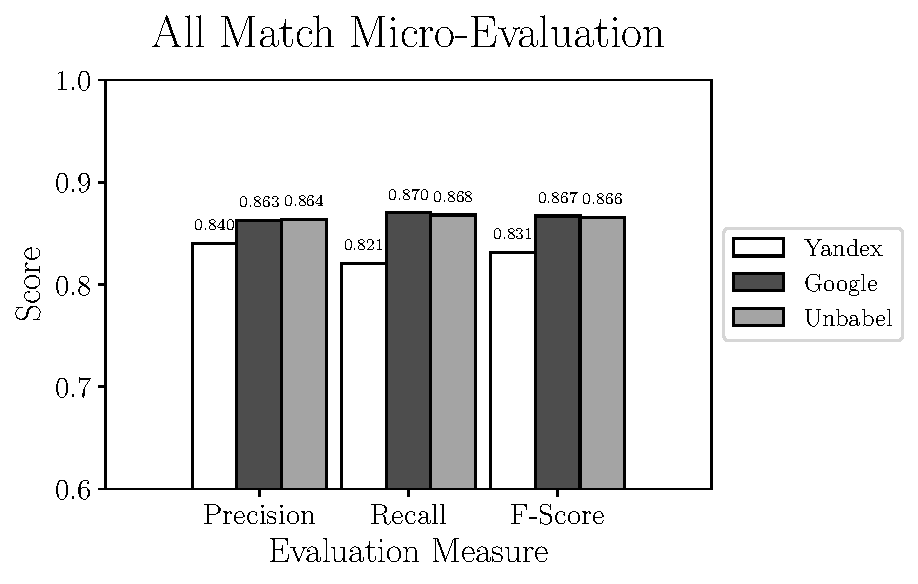
\includegraphics[width=0.9\textwidth]{SupportFiles/plots/all_match_micro_total_plot.pdf}
	\caption{Micro Evaluation of Translations being tested (All Match)}
	\label{fig:micro_eval_all}
\end{figure}

\begin{figure}
	\centering
	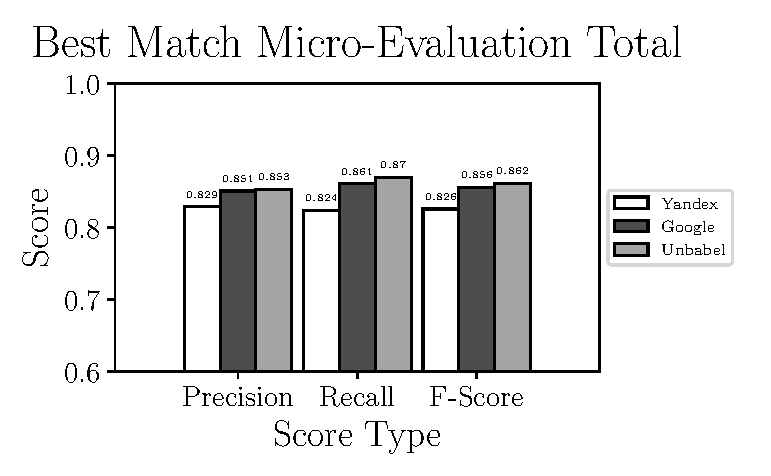
\includegraphics[width=0.9\textwidth]{SupportFiles/plots/best_match_micro_total_plot.pdf}
	\caption{Micro Evaluation of Translations being tested (Best Match)}
	\label{fig:micro_eval_best}
\end{figure}

\begin{figure}
	\centering
	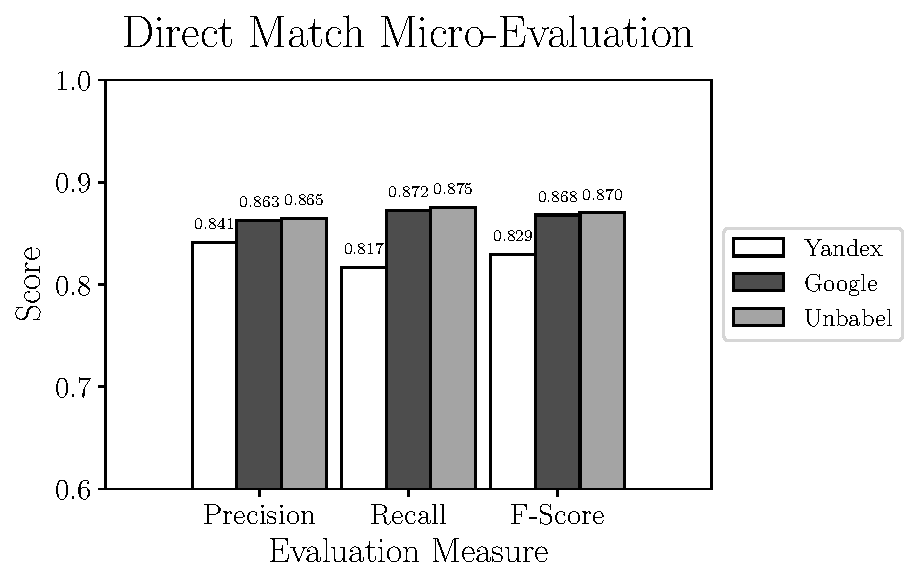
\includegraphics[width=0.9\textwidth]{SupportFiles/plots/direct_match_micro_total_plot.pdf}
	\caption{Micro Evaluation of Translations being tested (Direct Match)}
	\label{fig:micro_eval_direct}
\end{figure}



As seen in Figures \ref{fig:micro_eval_all}, \ref{fig:micro_eval_best} and \ref{fig:micro_eval_direct} (Supplementary Table 1 presents the data in table format), the terms extracted from Google translations are more similar to the ones extracted from HT translations than the ones from Yandex translations. This could be just because the human translators used Google Translator to help them in their translation process. This argument loses strength if we assume Google Translate translation outputs changed since the articles were human translated (publication years of the articles used range from 2003 to 2013), but data could not be found to corroborate this assumption. 

The terms extracted from Unbabel and Google translations are really similar, the F-Scores being almost equal. That the translations are similar is not too surprising since the Post-Editing phase at Unbabel is done after MT translation using Google. What could be surprising is that Unbabel does not have a higher score. One conclusion to take from this is that Post-Editing step on the MT+PE does not add value for this task. The results are similar when a Macro Evaluation is done (see Supplementary Table 2).

In the Introduction to the thesis I've proposed the following hypothesis:

\begin{description}
	\item[Hypothesis:] MT+PE is a good trade-off between quality and cost, compared with MT and HT, for translating Portuguese Radiology reports to English, for the purpose of identifying RadLex terms in the translated text. 
\end{description}

I've written that for this to be true, "The terms extracted from MT+PE translations have to be more similar to the ones extracted from the HT translation than the ones extracted from MT translations". This does not hold. So, for this task, if someone had to choose between Google and Unbabel, this someone would be better off using Google since it is cheaper. 

I've also written that for the hypothesis to be true, "The terms extracted from MT+PE translations have to be similar enough to the ones extracted from the HT translation". The terms extracted from any of these translations are not extremely different but they are also not equivalent to the ones extracted from the human translation. It could be the case that for some applications only translations close to human quality are acceptable, while for other applications a mediocre translation would be good enough. Therefore, the suitability of the MT and MT+PE translations probably depends on the practical usage for these translations and annotations. 

To better understand the results I will now provide a detailed analysis on the annotations for the "clinical finding" and "anatomical entity" subtrees of RadLex. These are two of the subtrees that probably would be more important when applying RadLex to a Information Retrieval system, a type of application for which the results of this study can be useful.

\subsection{Clinical Finding and Anatomical Entity Subtrees}

\begin{figure}
	\centering
	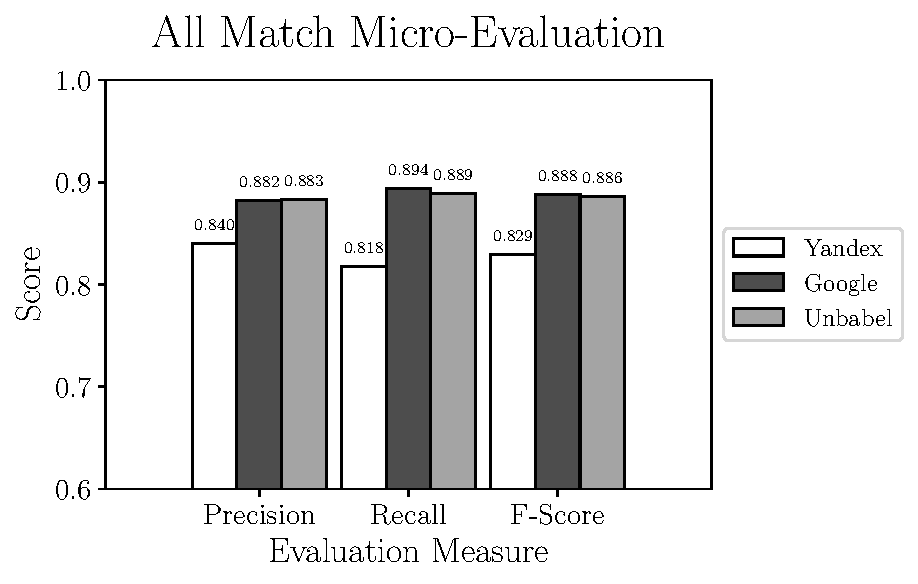
\includegraphics[width=0.9\textwidth]{SupportFiles/plots/all_match_micro_clinical_anatomical_subtrees_plot.pdf}
	\caption{Micro Evaluation of translations being tested, considering just the terms from RadLex "clinical finding" and "anatomical entity subtrees" (All Match)}
	\label{fig:micro_eval_subtrees_all}
\end{figure}


\begin{figure}
	\centering
	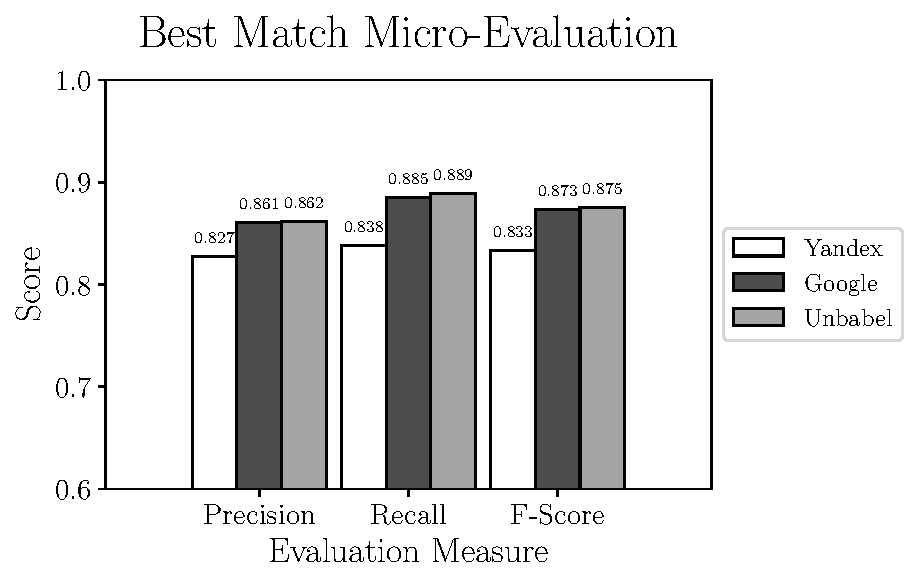
\includegraphics[width=0.9\textwidth]{SupportFiles/plots/best_match_micro_clinical_anatomical_subtrees_plot.pdf}
	\caption{Micro Evaluation of translations being tested, considering just the terms from RadLex "clinical finding" and "anatomical entity subtrees" (Best Match)}
	\label{fig:micro_eval_subtrees_best}
\end{figure}


\begin{figure}
	\centering
	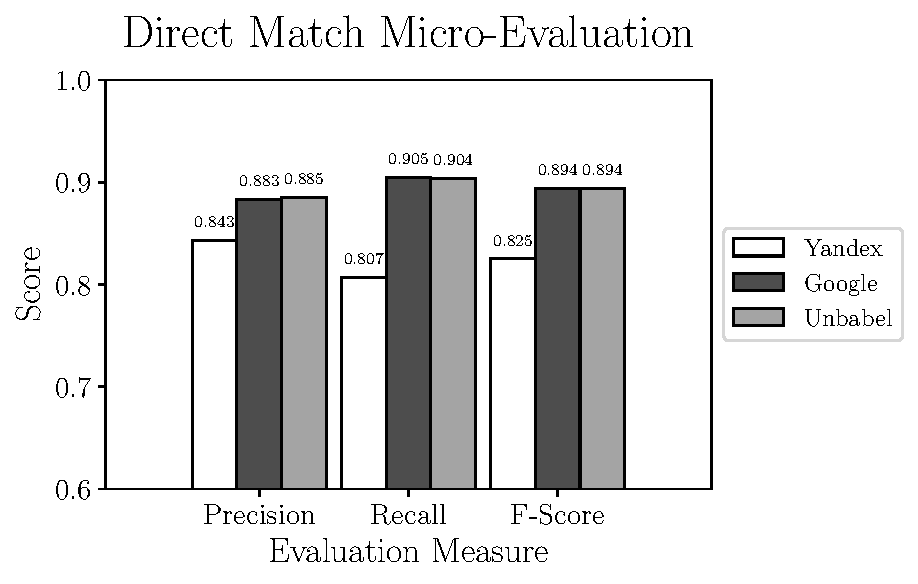
\includegraphics[width=0.9\textwidth]{SupportFiles/plots/direct_match_micro_clinical_anatomical_subtrees_plot.pdf}
	\caption{Micro Evaluation of translations being tested, considering just the terms from RadLex "clinical finding" and "anatomical entity subtrees" (Direct Match)}
	\label{fig:micro_eval_subtrees_direct}
\end{figure}

Depending on the type of annotation approach and translation it was found between 35.25 and 55.55 "clinical finding" or "anatomical entity" terms per document (See Supplementary Table 3). As seen in Figures \ref{fig:micro_eval_subtrees_all}, \ref{fig:micro_eval_subtrees_best} and \ref{fig:micro_eval_subtrees_direct} (see Supplementary Table 4 to see the data in table format), the scores obtained are similar to the ones obtained for all terms, with Yandex translation extracted terms being the less similar to the HT translation extracted terms and Google and Unbabel having similar scores. Similar results were found when Macro evaluation was performed (see Supplementary Table 5). But why these scores? 

In an attempt to better understand the results, we done an analysis of the False Positives and False Negatives errors committed by the MT and MT+PE translations, focusing on the terms belonging to the "clinical finding" or "anatomical entity" RadLex subtrees. From preliminary analysis we knew that some of the FPs and FNs are not caused by a erroneous translation but due to other causes, for example, an alternative translation which is correct but causes a different annotation, e.g., translating parênquima pulmonar to pulmonary parenchyma instead of to lung parenchyma. Both translations are correct but the second one leads to the extraction of the term lung while the first does not. Still, we expected a higher number of real translation errors using Yandex compared with the Unbabel or Google translations, since both of these types of translation had better scores.

I did an analysis on the FPs and FNs errors committed by Yandex, Google and Unbabel translations in 9 random documents and each error was classified by type (See Supplementary Table 6). The results from the Best Match Approach were used. As predicted, the percentage of errors of Yandex due to a wrong translation (25\% of 100 FPs or FNs) was higher than the percentage of errors of Google and Unbabel (22.09\% of 86 and 21.18\% of 85 FPs or FNs, correspondingly), but only slightly (See Supplementary Tables 7 and 8). The reasons for the others FPs and FNs included, among others, cases i) of different translations which are both correct but lead to different annotations, as described above and ii) in which the word extracted does not have the same meaning in the text as it has in RadLex. For example, the case of extracting the anatomical term \textit{hand} from "(...) on the other hand, it has to be considered that (...)" , in which the word \textit{hand} is used metaphorically. This happens because a rule-based approach is being used, which does not consider the context of the term. 

There were a lot of these ii) cases, which maybe would happen less if a Machine Learning NER approach was used. We thought about this but the problem is that, to the best of our knowledge, there is no data  readily available to conduct an experiment of this type, i.e., we could not find English Radiology text resulting from human translation of Portuguese text and annotated with RadLex terms by experts. 

Next I analyzed what kind of real translation errors were causing the FPs and FNs (See Supplementary Table 9). These subcategories included cases in which:

\begin{itemize}
	\item There was an extra word in the translation;
	\item There was a missing word in the translation;
	\item A wrong hyphenation was used;
	\item An acronym was not translated; 
	\item The test translation used a term that was too general;
	\item A wrong lexical variation was used;
	\item The most correct medical term was not used;
\end{itemize}

Each of these cases had a low number of occurrences and so it is not worth a deeper analysis. One interesting thing to note is that in the Yandex translations there were some cases (six) in which the original Portuguese word was not even translated. This never happened in the Google and Unbabel translations that were analyzed. This could be explained by the fact that probably Yandex focuses on different languages than Google and so their Portuguese-English translation and/or language models are not so well trained. But most of the errors correspond to just to a general wrong choice of terms to use as a translation. For example, translating \textit{média} to \textit{middle} instead of \textit{mean} or \textit{lesões de via biliar} to \textit{lesions via bile} instead of \textit{lesions to the biliary tract}. This type of problems could probably be solved by training Google and Yandex models with more data, specifically data related to medicine.

One could expect that Unbabel translations would have a lot less mistakes than Google's but this is not always the case. There are situations where errors are even added during the Post-Editing step. A review of the errors makes us propose that this could be due to the lack of medical knowledge of Unbabel current editors. For example, a stroke is something that occurs in the brain but in one case it was used as something that happens in the heart - someone with some knowledge on medicine would not make this error. But the truth is that Unbabel currently do not have a focus on medical content. I predict that if they did and invested in growing a crowd of experts with a better knowledge of medical language, this would lead to better results.


  
